\newcommand{\tttt}{Vectoren}
\newcommand{\dddd}{Datum 1}

\documentclass{article}
\usepackage[utf8]{inputenc}

\usepackage{listings}
\usepackage{color}
\usepackage{amsmath}
\usepackage{wrapfig}
\usepackage{graphicx}
\graphicspath{ {./images/} }
\usepackage{tikz}

\definecolor{mygreen}{rgb}{0,0.6,0}
\definecolor{mygray}{rgb}{0.5,0.5,0.5}
\definecolor{mymauve}{rgb}{0.58,0,0.82}

\lstset{ %
  backgroundcolor=\color{white},   % choose the background color
  basicstyle=\footnotesize,        % size of fonts used for the code
  breaklines=true,                 % automatic line breaking only at whitespace
  captionpos=b,                    % sets the caption-position to bottom
  commentstyle=\color{mygreen},    % comment style
  escapeinside={\%*}{*)},          % if you want to add LaTeX within your code
  keywordstyle=\color{blue},       % keyword style
  stringstyle=\color{mymauve},     % string literal style
  numbers=left,               % Ort der Zeilennummern
  language=java,
}

\begin{document}

\title{\tttt}
\author{Steven Bronsveld}

\maketitle
\section{Gegevens}
Uiterlijke inleverdatum: \textbf{\dddd}
\subsection{Links}
\begin{itemize}
    \item Github.com/StevenBrons 
    \item https://natureofcode.com/book
    \item http://hello.processing.org/editor/
\end{itemize}


\newpage


\section{Leerdoelen}
\begin{itemize}
	\item \texttt{x,y} co\"ordinaten om kunnen zetten in de \texttt{PVector} objecten.
	\item Gebruik kunnen maken van de volgende PVector methods: \texttt{add(PVector p), sub(PVector p), mult(float amount), rotate(float angle)}
\end{itemize}

\section{Uitleg}
\begin{itemize}
\item\href{https://natureofcode.com/book/chapter-1-vectors/}{Nature Of Code Chapter 1} Alleen \textbf{1.1, 1.2, 1.3, 1.4, 1.5}
\item\href{https://www.youtube.com/watch?v=mWJkvxQXIa8&list=PLRqwX-V7Uu6ZwSmtE13iJBcoI-r4y7iEc}{Vectors - The Nature of Code} Alleen \textbf{1.1, 1.2, 1.3, 1.4}
\end{itemize}

\section{Vectoren}
Omdat het onhandig is om telkens twee argumenten mee te moeten geven voor een positie op het scherm \texttt{int x, int y} en we een betere manier nodig hebben om met co\"ordinaten om te gaan bestaat er in Processing de \texttt{PVector} class.

\subsection{[optioneel] Vectoren in de wiskunde}
Een vector is een verzameling van meerdere variabelen. Wij zullen ons alleen maar bezig houden met 2 dimensionale vectoren van \texttt{x,y} co\"ordinaten.
Een vector wordt als volgt genoteerd: 
$$
\vec{v}=
\begin{pmatrix}
2\\ 
3
\end{pmatrix}
$$
Er zijn een paar rekenregels, die erg voor de hand liggen als je bedenkt dat een vector gewoon een verzameling van twee co\"ordinaten is:
$$
\begin{pmatrix}
a\\ 
b
\end{pmatrix}
+
\begin{pmatrix}
c\\ 
d
\end{pmatrix}
=
\begin{pmatrix}
a + c\\ 
b + d
\end{pmatrix}
$$
$$
a * 
\begin{pmatrix}
b\\ 
c
\end{pmatrix}
=
\begin{pmatrix}
a*b\\ 
a*c
\end{pmatrix}
$$
De tweede rekenregel heet \textit{scalaire vermenigvuldiging}. Dit geeft het uitrekken of inkrimpen van een vector weer. Dit is makkelijker te zien als we de vectoren als pijltjes (of natuurkundige krachten) tekenen:\\
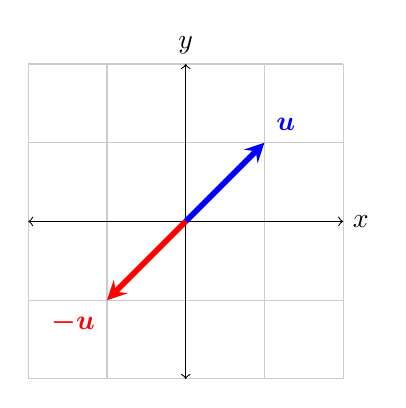
\begin{tikzpicture}
  \draw[thin,gray!40] (-2,-2) grid (2,2);
  \draw[<->] (-2,0)--(2,0) node[right]{$x$};
  \draw[<->] (0,-2)--(0,2) node[above]{$y$};
  \draw[line width=2pt,blue,-stealth](0,0)--(1,1) node[anchor=south west]{$\boldsymbol{u}$};
  \draw[line width=2pt,red,-stealth](0,0)--(-1,-1) node[anchor=north east]{$\boldsymbol{-u}$};
\end{tikzpicture}
\subsubsection{Opdrachten}
\begin{enumerate}
	\item Teken de optelling van $\begin{pmatrix}2\\1\end{pmatrix}+\begin{pmatrix}-1\\3\end{pmatrix}$
	\item Bereken $2*((3*\vec{a})+\vec{b})$ met $\vec{a}=\begin{pmatrix}1\\2\end{pmatrix}$ en $\vec{b} = \begin{pmatrix}-1\\2\end{pmatrix}$
	\item Bepaal het midden tussen $\vec{a}$ en $\vec{b}$. (We zoeken dus een algemene formule voor het midden tussen twee vectoren).
	\item Bereken de vector op $\frac{2}{3}$ afstand tussen $\vec{a}$ en $\vec{b}$ (Wederom zoeken we dus een algemene formule).
\end{enumerate}

\subsection{PVector}
Processing heeft de class \texttt{PVector}, met daarin een heleboel handige methods, zie \texttt{https://processing.org/reference/PVector.html}
\begin{lstlisting}
	void setup() {
		PVector v1 = new PVector(3,2);
		PVector v2 = v1.copy();
		v1.add(v2);
		v2.sub(new PVector(1,1));
		v1.mult(3);
		drawDot(v1);
		drawDot(v2);
	}
	
	void drawDot(PVector v) {
		circle(v.x,v.y,5);
	}
\end{lstlisting}
\textbf{Let op! De oorsprong (0,0) zit bij computers links boven, en niet links onder zoals bij de meeste wiskundige grafieken! De y-as is als het ware gespiegeld!}\\
Op welke co\"ordinaten tekent dit stukje code een stip?
Schrijf je antwoord in een \textit{comment} van je sketch:

\subsection{Polygoon}
Een gelijkzijdige polygoon of veelhoek is een figuur met \texttt{n} hoeken en lijnstukken van gelijke lengte. Voor \texttt{n = 3} is dit een \textit{driehoek}, voor \texttt{n = 4} is dit een \textit{vierkant}, voor \texttt{n = 5} is dit een \textit{pentagon} en voor \texttt{n = 17} is dit een \textit{heptadecagoon}. Maak de volgende functie:
\begin{lstlisting}
	void polygon(PVector center, int radius, int n) {
	}
\end{lstlisting}
Deze functie moet een polygoon van \texttt{int n} hoeken tekenen met een straal van \texttt{int radius}. Maak gebruik van vectoren en gebruik de \texttt{rotate(float angle)} method. \\
\textbf{Let op!} Een hoek wordt niet in graden uitgedrukt maar in radialen, dit betekent dat \'e\'en cirkel (dus 360 graden) gelijk is aan $2 * \pi$, ofwel: \texttt{2 * PI}.
\begin{figure}[h!]
	\centering
	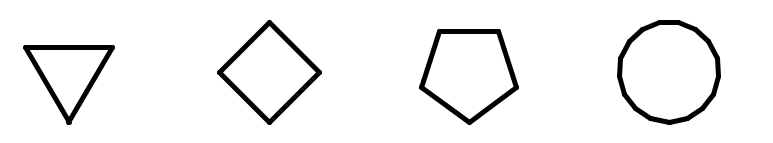
\includegraphics[width=\textwidth]{polygon.png}
	\label{fig:polygon}
	\caption{Polygonen met n = 3, 4, 5 en 17}
\end{figure}


\section{Middelloodlijn}
Maak de volgende functie aan:
\begin{lstlisting}
	void bisector(PVector p1, PVector p2) {
	}
\end{lstlisting}
Deze functie moet de middelloodlijn tekenen van de twee functies met de lengte gelijk aan de afstand tussen de twee functies (zie figuur \ref{fig:bisector}). \textbf{Tip:} Probeer eerst op papier een aantal middelloodlijnen te tekenen en probeer vervolgens om de twee punten waartussen de lijn getrokken moet worden te vinden.
\begin{figure}[h!]
	\centering
	
\includegraphics[width=4cm]{bisector.png}
	\label{fig:bisector}
	\caption{Middelloodlijn, de twee stippen geven \texttt{p1} en \texttt{p2} aan}
\end{figure}


\section{Koch's Curve gen0}
Maak de functie
\begin{lstlisting}
	void kochCurve(PVector p1, PVector p2) {
	}
\end{lstlisting}
Deze functie tekent de volgende figuur tussen \texttt{p1} en \texttt{p2}:
\begin{figure}[h!]
	\centering
	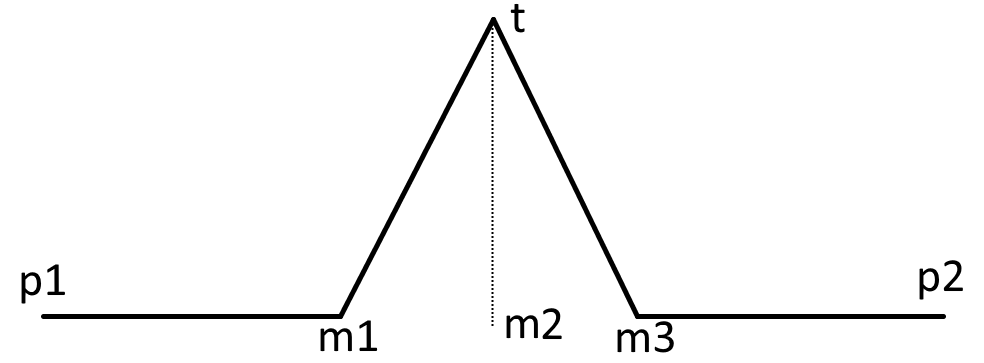
\includegraphics[width=\textwidth]{koch.png}
	\label{fig:koch}
	\caption{Koch's curve gen 0}
\end{figure}
Hierbij ligt \texttt{m2} midden tussen \texttt{p1} en \texttt{p2}.\\
De afstand tussen \texttt{p1} en \texttt{m1} is even groot als de afstand tussen \texttt{m2} en \texttt{t}.\\
\texttt{m1} ligt op $\frac{1}{3}$ afstand van \texttt{p1} naar \texttt{p2}.\\
\texttt{m3} ligt op $\frac{2}{3}$ afstand van \texttt{p1} naar \texttt{p2}.\\
\textbf{Tip:} Dit is een redelijk complexe opdracht. Teken dit eerst uit, en probeer al voordat je begint met coderen te weten \textit{wat} je precies gaat coderen. Maak gebruik van de \texttt{dist} \texttt{rotate} en \texttt{mult} PVector methods.

\section{[Bonus] Hilbert's Curve}
Maak de volgende functie:
\begin{lstlisting}
	void hilbertCurve(PVector p1,PVector p2) {
	} 
\end{lstlisting}
Die de volgende figuur tekent:
\begin{figure}[h!]
	\centering
	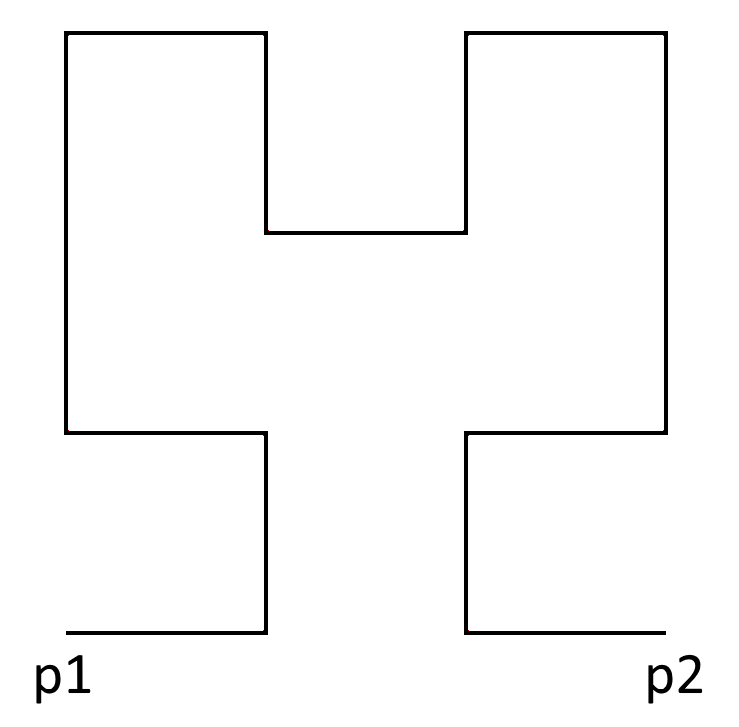
\includegraphics[width=4cm]{hilbert.png}
	\label{fig:koch}
	\caption{Hilbert's Curve}
\end{figure}

\section{Inleveren}
Als je klaar bent met de hele opdracht kun je deze naar je \textit{repository} \texttt{pushen}.



\end{document}
